\documentclass[upright, contnum]{lib/umemoria}

\depto{DEPARTAMENTO DE CIENCIAS DE LA COMPUTACIÓN}
\author{PABLO IGNACIO ESTEFO CARRASCO}
\title{REESTRUCTURACIÓN Y REFACTORIZACIÓN DE UNIT TESTS CON TESTSURGEON}
%\auspicio{.}
\date{JULIO 2013}
\guia{ALEXANDRE BERGEL}
\carrera{TÍTULO DE INGENIERO CIVIL EN COMPUTACIÓN}
\comision{ROMAIN ROBBES}{JOSÉ PINO URTUBIA}{\ }

%\usepackage{lipsum}

%\usepackage[latin1]{inputenc}
%\usepackage[T1]{fontenc}
% Niveles de produndidad para mostrar
\setcounter{secnumdepth}{4}
\setcounter{tocdepth}{4}
\usepackage{float} %== Imagenes


\begin{document}

\frontmatter
\maketitle

%% Preliminary
\begin{abstract}

% Problema
\par Actualmente la actividad de Testing es fundamental dentro del ciclo de desarrollo de cualquier proyecto de software serio. Es más, las metodologías ágiles elevan su relevancia dentro de la construcción del software a tal nivel que está prohibido añadir una nueva funcionalidad sin que se haya escrito previamente un test que la valide.

% Relevancia
\par A medida que el software crece en funcionalidades y cambian los requerimientos se vuelve más complejo. Es por eso que existen varias técnicas para restructurar el código para hacerlo más flexible a los cambios y permitir que crezca. 

\par Sin embargo, los test también crecen en número y en complejidad. Escenario en el cual abundan problemas de redundancia tanto en el código fuente de éstos como en su ejecución. Pero, a difernecia con el código ``funcional'', poco esfuerzo se ha realizado por parte de la industria y la academia para mantener una estructura y diseño limpio de los tests. 

\par Una de las consecuencias importantes de este problema es el gran tiempo que toma ejecutar todos los tests. Al tener tests redundantes, la ejecución tarda más tiempo del necesario lo hace que los desarrolladores disminuyan la frecuencia de la ejecución de estos, e inclusive minimicen la cobertura de sus tests. Esto último atenta críticamente en la confiabilidad del código funcional y por ende de la aplicación completa.

\par En este trabajo se propone una herramienta para detectar problemas de diseño de los tests o \emph{test smells}. \emph{TestSurgeon} aborda este problema desde distintos aspectos de análsis de un test, tales como: su código fuente y su ejecución. A través de una intuitiva intefaz, el desarrollador puede navegar sobre las pruebas unitarias y realizar comparaciones entre tests ayudado por métricas dedicadas que lo guían para encontrar casos interesantes de posible restructuración. Además provee una completa visualización que condensa armónicamente una serie de métricas que describen y a su vez diferencian la ejecución de dos tests. Esto permite realizar un análisis comparativo eficaz entre dos tests. De esta manera, TestSurgeon permite detectar diferencias semánticas entre tests y encontrar redundancias entre estos para una posterior refactorización.

\par Se presenta también en detalle una experiencia de la aplicación de \emph{TestSurgeon} sobre los tests de \emph{Roassal}, un motor de visualización ágil. Se detallan tres escenarios de refactorización y restructuración de test que la herramienta permite detectar.  
% Este problema es particularmente importante cuando se automatiza el proceso de liberación de código a través de integración contínua. Donde antes de liberar una nueva funcionalidad se ejecutan todos los tests para verificar que no se ha roto ninguna funcionalidad previamente liberada. Por tanto, el tener tests redundantes tiempo valioso se pierde y provoca disminución en la velocidad del equipo de desarrollo.  

% Approach
\par 

% Resultados

% Conclusiones




\end{abstract}
\begin{dedicatoria}
Por mi y por todos mis compañeros.
\end{dedicatoria}
\begin{thanks}
Vale cabros :D
\end{thanks}

%\cleardoublepage
\tableofcontents
%\cleardoublepage
\listoftables
%\cleardoublepage
\listoffigures

\mainmatter

%% Chapters
\chapter{Introducción} 
%% Intro
\par 
Dado la naturaleza de este tipo de código, su estudio e investigación ha intentado principalmente mejorar su efectividad para hacer software cada vez más confiables. Sin embargo, el problema diseño y mantención del código de test lleva bastante tiempo sin ser enfrentado en forma correcta y con la profundidad necesaria. 


%% Terminologia
\section{Terminología}

\par Para la lectura adecuada del documento, se presenta la siguiente terminología con los conceptos fundamentales que se utilizarán a lo largo del documento:

\begin{description}
\item[\emph{test}]: corresponde a un trozo de código que tiene como finalidad simular un comportamiento particular de alguna componente o compontentes del sistema para realizar verificaciones que validen el comportamiento esperado de estas. También se le nombra: \emph{método de test}, \emph{test method} o \emph{prueba de software}.
\item[\emph{unit test}]: corresponde a un grupo de tests que, en conjunto, verifican una funcionalidad en común. También se le nombra: \emph{prueba unitaria} o \emph{grupo de tests}
\item[\emph{smell}]: se refiere a una deficiencia en el diseño del código que da pie a problemas en su mantenibilidad y/o extensibilidad. Cuando existen smells sobre el código se pruebas se nombra como un \emph{test smell}.
\end{description}

%% Motivacion

% - Contexto: Práctica de Testing, Unit Testing
% Los test juegan un papel clave en la confiabilidad de 
% - Relevancia del Problema: Mantenibilidad

% - Alternativas de la Solución

% - Descripción de la solución (muy general)

%% Objetivos
\section{Objetivos}
\par El objetivo general de este trabajo es crear una herramienta que permita a los desarrolladores refactorizar y reestructurar sus test de una manera más fácil y mejorar la performance de estos.

\subsection*{Objetivos Específicos}
\begin{itemize}
\item Identificación de las métricas relevantes para caracterización de tests methods desde el punto de vista de un análisis dinámico
\item Desarrollar una visualización que permita detectar redundancia y solapamiento entre grupos de test methods (o unit tests)
\item Investigar refactorizaciones automáticas y semi-automáticas para unit tests y sus implicancias en performance y cobertura
\item Desarrollar una interfaz gráfica efectiva y usable para el uso cotidiano dentro del desarrollo de software
\end{itemize}

%% Organizacion del documento
\section{Estructura del documento}

\par En el \chapref{espec-prob} se presenta el problema de la mantenibilidad de tests en detalle, su contexto y relevancia. Posteriormente se presenta el marco teórico que entrega los conceptos técnicos necesarios (\secref{marco-teorico}), y se entregan una seria de antecedentes que muestra el trabajo realizado tanto por la academia como por la industria en sobre el problema de diseño del código de tests se refiere (\secref{trabajo-relacionado}). 

\par Luego, con la base conceptual y contextual del problema presente, se describe en detalle la solución propuesta: \emph{TestSurgeon}. Primero en forma conceptual en el \chapref{descripcion-solucion} y después en forma técnica en el \chapref{implementacion}. Y después, en el \chaplabel{caso-de-estudio} se muestra una aplicación de la herramienta con una serie de descubrimientos interesantes. 

\par Finalmente en el \chapref{conclusion} se revisa el cumplimiento de los objetivos planteados, las conclusiones del trabajo así como también las posibilidades y algunas directrices para continuarlo.

\par Se adjuntan también algunos anexos interesantes que complementan el documento y entregan datos que por su extensión no pudieron incluídos directamente en los capítulos.

\chapter{Especificación del Problema}\chaplabel{espec-prob}
% Conceptos para que el lector entienda y pueda leer depsués



\section{Contexto: Test como ``conductores'' del diseño}
\par Durante el desarrollo de un software una de las actividades principales es el testeo de los requerimientos. Existen variadas técnicas, metodologías y artefactos relacionados a esta actividad. En particular, la creación de pruebas automatizadas es una práctica cotidiana en cualquier proyecto de software y comprende parte importante de los artefactos generados. \\

\par En particular, los proyectos de software ágiles dan gran importancia a estos artefactos, ya que cada historia de usuario (requerimiento) debe tener pruebas de aceptación (tests de alto nivel). Estos se escriben y detallan en conjunto con el cliente para asegurar que el código que se creará cumple lo que éste pide: ni menos ni más.

\par Estas historias de usuario están escritas en lenguaje natural por lo que se deben \emph{transcribir} al lenguaje técnico: código fuente. Entonces, antes de escribir una funcionalidad, los desarrolladores crean los tests: código fuente que garantiza que una característica se comporta como es requerida. Este proceso se denomina \emph{Test-Driven Development} (o TDD)~\cite{Beck02a}  o Desarrollo Dirigido por Pruebas: se escribe el test, se ejecuta y este falla (ya que no se ha escrito el código que suple dicha característica). Luego se escriben las clases y métodos que hace que el test funcione, éste se vuelve a ejecutar y esta vez ``pasa''. Finalmente se refactoriza el código recién escrito para mantener un diseño limpio y mantenible en el tiempo.

\par Esta práctica está dentro del núcleo de la filosofía que enmarca la agilidad a tal nivel que está prohibido agregar una nueva funcionalidad sin, previamente, haber escrito un test que lo valide~\cite{Beck02a}. Esta queda documentado en el libro de Robert Cecil Martin (más conocido como``Uncle Bob'')~\cite{Mart02b} uno de los escritores del manifiesto ágil~\cite{Fowl01a} quien declara:

\begin{quote}
\emph{``The iteration between writing test cases and code is very rapid [...]. As a result, a very complete body of test cases grows along with the code.''}
\end{quote}


\par En la práctica, aplicando TDD se obtiene una gran cantidad de pruebas unitarias (unit tests) que representan los casos de prueba de la aplicación (Test Cases). Cada Unit Test contiene varios métodos de tests (test methods) que cubren los distintos aspectos a verificar en la funcionalidad que se está testeando.


\section{Problema: ¿Cómo mantener los tests?}

\par La comunidad de ingeniería de software ha producido herramientas efectivas y buenas prácticas para lograr refactorizaciones en el código base que otorguen un buen diseño. Sin embargo, en cuanto al código de las pruebas de software no sucede en igual proporción. Es más, éstos son raramente modificados y carecen del cuidado que se le da al código base, sin pensar su modularidad ni extensibilidad. 

\par Por lo cual no es difícil encontrar deficiencias como \textbf{solapamientos} entre test methods o más general, entre test cases. Estos solapamientos pueden ser de carácter estático ( duplicación de código ), o bien dinámicos, es decir que dos test methods tienen ejecuciones similares y por consiguiente representan una ineficiencia de tiempo.

\par Estas deficiencias en el diseño y calidad del código de las pruebas unitarias tienen consecuencias importantes en la calidad del código testeado y en el mismo proceso de desarrollo:
\begin{itemize}
\item \textbf{Rendimiento} Debido a los solapamientos previamente mencionados, muchas veces existe \textbf{ejecución redundante} que va en contra de las características deseables de una suite de tests. Muchas veces los tests dejan de ejecutarse con la frecuencia necesaria.
\item \textbf{Depuración}\footnote{o \emph{Debugging}.} Otra deficiencia conocida es que al correr los tests en presencia de un \emph{bug}, éste queda en evidencia por muchos tests, lo cual dificulta la identificación de su causa y su corrección. Coloquialmente se hace más difícil responder la pregunta: \emph{¿Cuál test miro primero?}
\end{itemize}
 
\par De esta manera, la confiabilidad en el producto y su calidad se ven impactadas negativamente. 

\par Un caso muy claro de la influencia del mal diseño y poco cuidado en los tests ocurre cuando el ciclo de desarrollo utiliza mecanismos de \textbf{Integración Contínua} (Continuous Integration). En esta práctica cada \emph{feature} se implementa tan pronto como es posible, se testea y se pasa a producción de inmediato. De esta manera el equipo de desarrollo realiza varias integraciones por día y el cliente obtiene rápidamente las nuevas funcionalidades a medida que las solicita. \\

\par A modo de ejemplo, la empresa MediaGeniX\footnote{MediaGeniX [en línea] \textless\url{http://www.mediagenix.tv}\textgreater [Consulta: 12/08/2013]} realiza la integración continua desde hace algunos años. Ahí, 30 desarrolladores trabajan sobre el mismo producto y cada uno de ellos construye varias versiones al día. Cada versión que se va a pasar a producción debe pasar su suite de pruebas que comprende alrededor de 30.000 tests. Ellos realizan 3 integraciones diarias en promedio, por lo cual recurren a técnicas de paralelización de ejecución de tests para lograrlo. Esto introduce un alto costo económico asociado al los recursos de hardware(servidores, clusters) y además un alto costo en tiempo. Esto se podría optimizar detectando redundancia en la ejecución. \\

% \par Esto evidencia la relevancia de mejorar la performance mediante la refactorización y restructuración de los unit tests.

\chapter{Antecedentes}


\section{Marco Teórico}\seclabel{marco-teorico}

\subsection{Profiling}

\par El \emph{Perfil de Ejecución} (o \emph{Execution Profiling}) es una forma de análisis dinámico que consiste en monitorear un software durante su ejecución para posteriormente analizar los datos obtenidos. Entonces los \emph{Profilers} son herramientas para ayudar a los ingenieros de software a recolectar datos durante la ejecución y analizarlos, y así poder determinar de mejor manera en qué parte de un sistema de software se gasta el tiempo de ejecución.


\par Para la obtención de datos, existen varias técnicas de profiling. Los principales son profiling por instrumentación (o \emph{Instrumentation-based profiling}) y a través de muestras (o \emph{Sampling-based profiling}). En la primera, se inserta código de instrumentación antes (instrumentación estática) o durante la ejecución (instrumentación dinámica). En la primera se agrega el código justo antes de ejecutar y por tanto la sobrecarga (o overhead) es menor. Sin embargo, cualquier código generado dinámicamente no será instrumentado. En tanto, la técnica basada en muestras aproxima el tiempo que se gastó en un método de la aplicación deteniendo el programa y guardando la colección de metodos que fueron ejecutados.

\par Usualmente los \emph{profilers} son utilizados con motivo de optimizar un sistema de software en cierto aspecto. Los datos a obtener a través de la técnica de profiling dependen completamente del problema a optimizar. Es por esto que el profiler a utilizar debe permitir la recolección de los datos necesarios con una mínima sobrecarga (o \emph{overhead}) para conseguir datos fidedignos y a la vez representativos. 

\par La herramienta de profiling escogida para en este trabajo es el framework \emph{Spy}, que utiliza la técnica de profiling basado en instrumentación del tipo dinámico. Spy está diseñado para analizar softwares en el contexto de orientación a objetos ya que se permite obtener métricas contextuales como: el número de ejecuciones de un método, cantidad de objetos instanciados de una clase, etc. Para mayor información sobre este y su implementación en \emph{TestSurgeon} ver la \secref{impl-spy}. 

\par Algunas de las aplicaciones exitosas basadas en Spy son \emph{Hapao}\footnote{Hapao [en línea] \textless\url{http://hapao.dcc.uchile.cl}\textgreater  [Consulta: 12/08/2013]}: una herramienta de cobertura de test desarrollada por Vanessa Peña y Alexandre Bergel~\cite{bergel2012increasing}, que permite gráficamente ver la cobertura de las clases y métodos contrastando la cobertura de los últimos con el grado de complejidad de éstos; y \emph{Kai}\footnote{Object Profile. Kai Profiler [en línea] \textless\url{http://www.objectprofile.com/\#/pages/products/kai/overview.html}\textgreater  [Consulta: 12/08/2013] }: un profiler que permite optimizar la ejecución de un software indicando, por ejemplo, dónde combiene incrustar una estructura de \emph{caching} para evitar redundancia de cálculo. En la \figref{hapao.png} y \figref{kai.png} se muestran capturas de pantalla de Hapao y Kai respectivamente.

\fig{h}{0.7}{hapao.png}{Ejemplo de la visualización de la cobertura de test en Hapao}
\fig{h}{0.7}{kai.png}{Diagnóstico de ejecución entregado por Kai}

\clearpage
%==========
\subsection{SUnit framework}

\par \emph{SUnit} es un framework de testing que apoya la creación de tests automatizados. SUnit es la implementación en Smalltalk del framework xUnit\footnote{la \textbf{x} se reemplaza por el lenguaje de programación, por ejemplo: jUnit para Java.} que de hecho historicamente es la primera. Las cualidades que caracterizan xUnit son:

\begin{itemize}
\item Los tests son repetibles: Cada test se puede ejecutar cuantas veces se quiera.
\item Los tests se ejecutan si necesidad intervención humana: Se puede dejar los tests ``corriendo'' durante la noche si necesidad de intervenir en su ejecución.
\item Los tests cuentan una historia: un test cubre al menos una funcionalidad del sistema. Un test entonces es un escenario que cualquier desarrollador puede leer para entender dicha funcionalidad.
\end{itemize}

\par En SUnit los tests están contenidos en clases llamadas unit tests. Los unit tests son clases que extienden o heredan de {\tt TestCase}, una de las clases arquitectónicas del framework. Los unit tests suelen nombrarse con el sufijo {\tt Test}, por ejemplo {\tt MarioBrosTest}. Los tests o test methods, por su parte se nombran con {\tt test} como prefijo, ejemplo {\tt testMarioFallDownAndLoseOneLife}.


\subsubsection{Arquitectura de \emph{SUnit}}
\par Estructuralmente, SUnit se compone de cuatro clases: {\tt TestSuite}, {\tt TestCase}, {\tt TestResource} y {\tt TestResult} como se muestra en \figref{sunit.pdf}. 
\begin{description}
\item[{\tt TestCase}] representa un unit test o una familia de test que comparten el mismo contexto. Esta clase está pensada para ser extendida por clases concretas. El contexto se especifica en el método {\tt setUp} donde las variables de instancia de cada subclase de {\tt TestCase} se inicializan y definen el contexto en el cual se ejecutará cada test. También se define el método {\tt tearDown} que es responsable de limpiar los objetos que hayan sido inicializados y modificados durante la ejecución del test para que pueden ser reinicializados por el método {\tt setUp}. Tanto {\tt setUp} como {\tt tearDown} son métodos abstractos. Entonces cada test se ejecuta de la siguiente manera:

\[ \texttt{setUp} \rightarrow \texttt{testMarioFallDownAndLoseOneLife} \rightarrow \texttt{tearDown} \]

\item[{\tt TestSuite}] contiene una colección de unit tests. Una instancia de {\tt TestSuite} está compuesto por instancias de subclases de {\tt TestCase} y {\tt TestSuite}. Las clases {\tt TestSuite} y {\tt TestCase} forman el patrón composite. 

\item[{\tt TestResult}] representa los resultados de una ejecución de {\tt TestSuite}. Contiene el número de tests que pasadon, el número de tests que fallaron y el número de errores.

\item[{\tt TestResource}] representa un recurso que es usado por un test o un conjunto de tests. Un recurso se asocia con una clase hija de {\tt TestCase} y se ejecuta automáticamente antes de la ejecución de todos los tests y una sola vez.   
\end{description}

\fig{h}{0.7}{sunit.pdf}{Las clases que representan el núcleo de \emph{SUnit}}

\subsubsection{Estructura de un test}
\par La estructura de cada test puede dividirse en dos partes: \emph{fixture} (o escenario) y \emph{assertions} (o verificaciones). En el fixture del test se crean e inicializan los objetos del escenario y se les hace interactuar a través de mensajes. No se considera parte del fixture todos los objetos inicializados y las operaciones realizadas en la ejecución del método {\tt setup}, aunque sí afectan la interacción en el fixture. Posteriormente, en el test hay una serie de validaciones o verificaciones, donde se comprueba el estado de los objetos a través de métodos verificadores heredados desde {\tt TestCase} tales como: {\tt assert:} para verificar una afirmación, {\tt deny:} para negarla, {\tt should:raise:} para verificar que una excepción en particular se lanzó, y {\tt shouldnt:raise:} para asegurar que no se lanzó cierta excepción.

\par A modo de ejemplo se muestra un código que bien podría ser un test básico del popular juego \emph{Super Mario Bros.}, donde un plomero de traje rojo va pasando por escenarios llenos de trampas y dificultades para poder llegar al castillo donde supuestamente está su princesa y rescatarla. Una de las trampas más comunes y sencillas del juego son hoyos de profundidad infinita donde Mario puede caer y perder una vida. En el ejemplo, inicializamos la variable local {\tt mario} con una instancia de la clase {\tt MBMario} que por defecto tiene 3 vidas\footnote{En la plataforma NES, Mario parte con 3 vidas.}. Luego lo insertamos al juego junto con un escenario en el cual, luego de dar tres pasos debiera caer a un hoyo y perder una vida. En el juego no se acaba sino hasta que a Mario se le acaban las vidas y vemos el mensaje de ``Game Over''. 

\begin{codeWithLineNumbers}
<i>MarioBrosTest>>testMarioFallDownAndLoseOneLife</i>
	" *--* Fixture *--* "
	| game mario scene |
	game := MBGame new.
	mario := MBMario new. " todos saben que Mario parte con 3 vidas"
	scene := #(#floor #floor #hole #floor). " un escenario con un hoyo en la tercera posicion"

	game setScene: scene.
	game setPlayer: mario.

	" hagamos a mario avanzar en el escenario"
	mario moveOneStep. 
	mario moveOneStep.
	mario moveOneStep. 
		
	" *--* Assertions *--* "
	
	self assert: (game currentPosition = #hole) "mario cayo al hoyo" 
	self assert: mario isDead. "deberia haber muerto puesto que cayo al hoyo"
	self assert: (mario lives = 2). "mario ahora tiene 2 vidas"
	self deny: game isGameOver. 
	

\end{codeWithLineNumbers}

\newpage
%=======
\section{Trabajo Relacionado}\seclabel{trabajo-relacionado}

\par A continuación se presenta una revisión de la literatura sobre el problema de mantenibilidad de las pruebas de software, y una revisión también de las herramientas de cobertura de test que abordan tangencialmente el problema.

\subsection{Revisión de la literatura}
\par Luego de revisar la bibliografía existente, entre los problemas con mayor investigación está la cobertura de los test: cómo medir y mejorar la cobertura del software testeado para aumentar la confiabilidad en éste; y  el testeo por mutación: como mejorar la efectividad de los test realizando variaciones en el código testeado que representan bugs y comprobar que test definidos atrapan o detectan esas anomalías. Con respecto al problema de mantenibilidad, las estrategias encontradas en la literatura corresponden a priorización de tests y comparación de tests, pero en volumen mucho menor a los tópicos mencionados anteriormente.

\par La priorización de tests y el \emph{clustering} son acercamientos populares para manejar el gran costo de correr una cantidad considerable de tests. Shin Yoo \etal~\cite{yoo2009clustering} han presentado un mecanismo para reducir las comparaciones 1-a-1 agruparlos y de esa manera facilitar la tarea humana de priorizar tests. Ellos crearon clusters de tests agrupándolos por similitud de ejecución. Cada ejecución fue representada por una cadena binaria donde cada dígito (1 o 0) representa si cierto método fue ejecutado durante ésta. Entonces, la similitud de cobertura es medida a través de una distancia binaria.

\par Vengala \etal~\cite{Vang09a} crearon un mecanismo para usar análisis estático y dinámico para optimizar las actividades de testing tales como \emph{selección de test}, \emph{eliminación de redundancia} y \emph{priorización de test}. Aunque sus métricas siguen el mismo espíritu que \emph{TestSurgeon}, están definidas para un ambiente de programación procedural lo cual es incompatible en un ambiente orientado a objetos.

\par Greiler \etal~\cite{Grei12a,greiler2012test} aborda el problema de entendimiento de tests suites proponiendo un framework sobre correlación entre similitud de test (Test Similarity Correlator). Este último produce una traza de ejecución que caracteriza la ejecución de los test a través de cuatro tipos de eventos: ejecución de un test method, evento de set-up y tear-down, ejecución de un método y lanzamiento de excepción. El entendimiento de test suites se realiza comparando las trazas de ejecución.

\par El código de test, desde el punto de vista de un artefacto de software tiene múltiples usos. Uno de ellos es documentación~\cite{Kuhn08a}. Especialmente para desarrolladores nuevos que tienen que enfrentarse con sistemas legados, los tests son altamente relevantes como ejemplos de código. Siguiendo esta perspectiva, Lienhard \etal~\cite{Lien08a} proponen una herramienta que facilita la tarea de escribir nuevos tests para esos sistemas a través de una visualización que llaman \emph{Test Blueprint}, como una guía para el entendimiento de los tests y el mantenimiento del código base.  

\par Reichhart \etal~\cite{reichhart2007rule} presenta \emph{TestLint}, una herramienta para determinar la calidad de los tests. En su trabajo presenta una aplicación de esta sobre una gran cantidad de unit tests obtenidos desde distintos repositorios open source. Además entrega una gran lista de \emph{test smells} de los cuales uno es analizado por \emph{TestSurgeon} y corresponde al escenario descrito en la \secref{escenario2}.

\par De los autores encontrados, el que aborda con mayor profundidad el problema de mantenibilidad en los tests es Markus Gaelli. Dentro de su investigación~\cite{gaelli2006composing,gaelli2007composing} presenta un estudio de clasificación de unit test~\cite{gaelli2005towards} representado por un arbol binario cuyas ramas indican cumplimiento de un criterio de clasificación. En este arbol, las hojas son los distintos tipos de test: Test donde se llama un solo método exactamente una sola vez(~50\% del total de tests estudiados), Test donde se llama un solo método en varios escenarios distintos (15\%), etc. Luego, utilizando esta taxonomía crea un metamodelo para escribir tests a través de ejemplos (o tests de alto nivel) a través de composiciones de tests más pequeños y de bajo nivel. Este modelo facilita la detección de errores ya que al componer tests, un bug en el código base sólo rompería uno de los tests de los que conforman el test ejecutado. Gaelli en su trabajo pretende en su trabajo promover la reutilización de tests de bajo nivel para crear ejemplos de funcionamiento, o tests de alto nivel. De esta generar ejemplos que sirven tanto como pruebas de software y documentación ejecutable~\cite{gaelli2006modeling}, acercando la brecha entre las unidades de software y las pruebas unitarias.

\subsection{Revisión de herramientas de cobertura de test existentes}

\par La gran cantidad de herramientas disponibles ilustra la importancia de la cobertura de tests para los profesionales de la industria. Se realizó una revisión de muchos de ellos incluyendo Emma, EclEmma, JCover, GroboCodeCoverage, JCoverage, Parasoft JTest, Purity Plus, Semantic Designs, TCAT, Quilt, NoUnit, InsectJ, Hansel, Gretel, Jester, JVMDI Code Coverage, JBlanket, Coverlipse, Koalog, Cobertura, Mojo y Thucydides. En el \apref{review-test-coverage-tools} se presenta la lista con las URL donde se puede obtener cada una de ellas. Esta recolección de las herramientas más populares se realizó a través de motores de búsqueda en la web, directorios de proyectos open source, descripciones de entornos de desarrollo y publicaciones científicas entre los que están: maven\footnote{Apache Maven Project [en línea] \textless\url{http://maven.apache.org/}\textgreater [Consulta: 12/08/2013]}, sourceforge\footnote{Sourceforge [en línea] \textless\url{http://sourceforge.net/}\textgreater [Consulta: 12/08/2013]}, github\footnote{GitHub [en línea] \textless\url{http://github.com/}\textgreater [Consulta: 12/08/2013]}, bitbucket\footnote{BitBucket [en línea] \textless\url{http://bitbucket.org}\textgreater [Consulta: 12/08/2013]} y el Eclipse marketplace\footnote{Eclipse Marketplace [en línea] \textless\url{http://marketplace.eclipse.org/}\textgreater [Consulta: 12/08/2013]}. 

\par Dentro de las 22 herramientas de cobertura de test estudiadas, solo 3 soportan un análisis comparativo de cobertura de test. 
\par JCover indica las variaciones de cobertura mostrando un gráfico tipo \emph{scatterplot} puntos representando los pares \emph{(version del software, \% cobertura)}. Al parecer TCAT compara tests, sin embargo no hay suficiente información publicada, de hecho, su sitio web no ha sido actualizado desde el año 2008. Jester realiza mutación a los tests para verificar cuán capaz es el unit test de capturar variaciones en el código base.


\chapter{Descripción de la Solución}\chaplabel{descripcion-solucion}




\section{Comparando la ejecución de tests con \emph{TestSurgeon}}

\par A la luz de los resultados del estudio comparativo entre el acercamiento al problema desde la perspectiva del análisis estático y análisis dinámico de  tests presentado en el \secref{exp-static-vs-dynamic}, se desprende que los tests deben ser analizados en base a lo que realmente ejecutan. Es por esto que se hace necesario que cualquier solución que apunte a abordar este problema, considere fuertemente un enfoque dinámico para el diagnóstico de la situación. Y también contrastarlo con el código fuente y otros aprontes de análisis estático para tener una visión más completa tanto del problema como de las alternativas de solución. 

\par En respuesta a este escenario, se presenta \emph{TestSurgeon}: un profiler para test unitarios. TestSurgeon realiza un monitoreo de la ejecución de test unitarios y recolecta datos sobre \emph{qué} está siendo testeado (cobertura) y \emph{cómo} (contexto de ejecución). TestSurgeon aproxima la similitud entre métodos de tests a través de una representación visual que relaciona el código testeado y métricas representativas que caracterizan (y diferencian) a los dos tests en comparación. 

\par El objetivo de TestSurgeon es apoyar a los ingenieros de software a reestructurar y refactorizar sus tests unitarios a través de un análisis sobre las diferencias de ejecución de los tests.

\subsection{Caso de uso}
\par A modo de resumen, para usar TestSurgeon se siguen las siguientes etapas: primero se lanza TestSurgeon sobre conjunto de paquetes, inmediatamente después se realiza el profiling sobre los paquetes seleccionados. Una vez finalizada esta etapa, se abre una ventana con el browser (o navegador) donde se escogen dos unit tests (no necesariamente distintos), posteriormente se seleccionan dos métodos de test pertenecientes a los unit tests escogidos. Finalmente se realiza la comparación entre los test methods seleccionados a través de la visualización y la zona de comparación de código. En TestSurgeon se realizan comparaciones de métodos de test uno-a-uno por lo cual, para diferenciarlos, se denominan \emph{test rojo} y \emph{test azul} en concordancia a los colores en la visualización.

\par Para ilustrar el uso de TestSurgeon se muestra a continuación un ejemplo sobre el software: \emph{Roassal}.

\par Un análisis con \emph{TestSurgeon} comienza lanzando el software desde una terminal de Pharo o \emph{Workspace} con el siguiente comando\footnote{Para más detalles sobre este comando y la implementación del browser ver la \secref{impl-browser} }: {\tt TSBrowser openOn: 'Roassal*'}. Este comando abre el browser y hace que se instrumenten todos los paquetes cuyo nombre comience con {\tt Roassal} (ej: {\tt Roassal-Core}, {\tt Roassal-Layout} o {\tt Roassal-Normalizers}, entre otros ).

\fig{h}{0.7}{caso-uso/1.png}{Lanzando el browser.}

\par Luego, TestSurgeon realiza un profiling sobre la ejecución de los tests encontrados en todos los paquetes de Roassal. Esto consiste en: ejecutarlos, recolectar datos y generar los objetos según el modelo de objetos de Spy(ver \secref{impl-spy}). Este proceso puede tardar desde unos segundos a algunos pocos minutos según la cantidad de tests encontrados y las operaciones propias dentro de cada test.

\par Una vez concluida la etapa de profiling, se despliega una ventana con cuatro zonas principales(ver \figref{caso-uso/2.png}): 
\begin{itemize}
\item {\bf Test Unitarios}: En la zona superior-izquierda aparecen dos listas. Se puede seleccionar solo un unit test por cada lista.
\item {\bf Métodos de Test}: Justo abajo de los test unitarios aparecen dos listas con los métodos de test de los unit tests seleccionados. En cada lista se pueden seleccionar un método. El método seleccionado de la izquierda se denomina \emph{test rojo} y el de la derecha \emph{test azul}.
\item {\bf Visualización}: Luego de seleccionados los tests rojo y azul se despliega una visualización que muestra la diferencia en la ejecución de ambos tests.
\item {\bf Código Fuente}: Junto con la visualización se muestra el código fuente de cada test.
\end{itemize}

\fig{h}{0.85}{caso-uso/2.png}{Zonas del browser de TestSurgeon.}

\par Primero se seleccionan los unit tests, uno por lista (Paso 1 y 2). De los unit tests escogidos, se debe seleccionar el test rojo en lista de la izquierda (Paso 3). Una vez seleccionado, la lista de métodos de test de la derecha se ordenan verticalmente según similitud de cobertura con respecto al test rojo (más similar arriba, más diferente abajo). La métrica de similitud por cobertura es la misma que se utilizó en el experimento de similitud estática contra similitud dinámica definida en la \secref{exp1-metricas-sim}. Esta facilita la búsqueda de casos interesantes a ser comparados. 

\par La cobertura, como métrica, no expresa el cómo los actores (objetos) se comportan (a través de métodos) mientras el test está siendo ejecutado. Por tanto se necesitan más datos~\cite{van2001refactoring,greiler2012test}. Entonces, una vez seleccionado el test azul (Paso 4) se puede realizar una mejor comparación observando una visualización (Paso 5) que justamente resalta las diferencias en la ejecución de ambos tests. Y finalmente contrastar (Paso 6) lo observado con el código fuente de ambos.


\fig{h}{0.9}{caso-uso/3.png}{Modo de uso del browser.}

%==========
\section{Visualización: \emph{Test Difference Blueprint}}\seclabel{test-diff-blueprint}

\par El objetivo de la visualización es comparar y encontrar las diferencias de ejecución que existen entre dos métodos de test. Para esto se utilizó intensivamente la gráfica de \emph{vistas polimétricas}~\cite{Lanz03d}, una técnica de visualización que permite identificar visualmente patrones en una gran masa de datos multidimensionales. Primero que todo, se debe hacer una comparación de la cobertura, es decir cuáles son los métodos y las clases testeadas por los métodos en comparación. Los elementos a visualizar, entonces, son las clases y sus métodos. 

%=============
\subsection{Clases y su jerarquía}

\par En la visualización se muestran todas las clases del código base que estén cubiertas por al menos uno de los dos tests en comparación. Las clases se presentan visualmente como grandes rectángulos con fondo blanco y borde negro. Estos rectángulos están unidos por líneas que hacen gráfica la relación de herencia entre estas. Como Pharo es un lenguaje orientado a objetos con herencia simple (cada clase puede heredar de una sola clase padre) desde una clase hija llega solo una línea, pero desde una clase padre pueden salir varias líneas a las clases que heredan directamente de ésta. TestSurgeon muestra entonces la jerarquía de clases a través de una distribución espacial de las clases, en forma de árbol (o \emph{tree layout}). De esta manera, la clase raíz (o la hereda de una clase que no está presente en los paquetes instrumentados) está en el tope superior de la imagen y en el siguiente nivel del árbol están las clases que heredan directamente de ésta, y así sucesivamente, formando un árbol.

% - Figura: Visualizacion jerarquia de clases
\fig{h}{0.7}{jerarquia-clases.pdf}{Jerarquía de la clase {\tt ROContainer}}

%=============
\subsection{Coloreando métodos para visualizar cobertura}\seclabel{viz-color}

\par Los elementos principales en el análisis, según el enfoque de TestSurgeon, son los métodos de las clases del código base. Los métodos están representados como rectángulos (o cuadrados) de menor tamaño posicionados dentro de la clase que lo define.  Los métodos heredados por la clase no están considerados en la visualización de dicha clase, sino que aparecen en la clase que lo define dentro de la jerarquía.  

\par Cada método tiene un color asignado:
\begin{itemize}
\item {\bf Rojo}: el método fue llamado únicamente durante la ejecución del test rojo.
\item {\bf Azul}: el método fue llamado únicamente durante la ejecución del test azul.
\item {\bf Gris}: el método fue ejecutado durante la ejecución de ambos tests.
\item {\bf Blanco}: el método no fue ejecutado.
\end{itemize}

\par Un aspecto importante dentro del análisis de cobertura es conocer los caminos de ejecución según las llamadas a métodos de una clase desde otro método definido en la misma clase. Estas llamadas son invocaciones a {\tt self} (o {\tt this} en Java) que permiten diferenciar si un método fue llamado directamente o a través de una invocación {\tt self} desde otro método. Para graficar esto se utilizó una distribución gráfica de Sugiyama~\cite{sugiyama1981methods} (o Sugiyama Layout). En el tope superior están los métodos que realizan mayores invocaciones a otro métodos definidos en la clase y que además no son invocados por otros métodos de la clase. En el tope inferior los métodos que no tienen invocaciones a otros métodos definidos en dicha clase pero sí son invocados por uno o más métodos definidos en la clase. Las invocaciones entre métodos están graficados por líneas rectas entre el método invocador y el invocado.

\par En una distribución de grilla y posicionados a la derecha dentro del rectángulo de la clase, están los que no tienen invocaciones a otros métodos definidos en dicha clase ni son invocados por métodos definidos en esa clase.

\fig{h}{0.4}{sugiyama-layout.pdf}{Ejemplo de Sugiyama Layout}

\par En la \figref{sugiyama-layout.pdf}, los métodos {\tt b} y {\tt c} son invocados en el método {\tt a}, es decir, en el cuerpo del método {\tt a} están las líneas {\tt self b} y {\tt self c}. Se puede apreciar que el test rojo ejecuta {\tt a}, {\tt b} y {\tt c}, y el test azul {\tt b} solamente. 

%=============
\subsection{Métricas para caracterizar la ejecución de los métodos }\seclabel{viz-metricas}

\par Hasta ahora, la visualización sólo grafica lo que ha sido ejecutado por uno, otro u ambos tests, es decir, la cobertura. Sin embargo este acercamiento no parece ser tan preciso ni suficiente\footnote{En el \secref{pq-cobertura} se explica a través de un ejemplo que efectivamente es necesaria más información que la cobertura para realizar una comparación efectiva.} para tener una idea real de cómo se ejecutaron dichos métodos. Allí es donde emerge la característica más distintiva e innovadora de la visualización de TestSurgeon: incorporar métricas que dan un contexto en el cual un método fue llamado durante la ejecución de los tests en comparación. Así no tan solo se visualiza cuáles fueron los métodos ejecutados por el test rojo o azul (o ambos) y cuáles no, sino que también muestra de qué manera tal método fue ejecutado y cuán distinta fue su ejecución entre ambos tests.

\par El \emph{Número de Llamadas} a un método ({\tt NOC} - Number of Calls, en inglés) es una de las dos métricas escogidas para esto. Tal como su nombre lo indica, representa la cantidad de veces que un método fue llamado para su ejecución. De esta manera, entre más veces fue llamado, más relevante es para ese test.

\par Por su parte, el \emph{Número de distintos objetos recibidores} de un método ({\tt NODR} - Number of Different Receivers, en inglés) indica cuántos objetos distintos ejecutaron dicho método. Esta métrica es particularmente útil cuando su {\tt NOC} es parecido ya que su {\tt NODR} puede ser distinto y así diferencia las ejecuciones del test rojo y azul ofreciendo una perspectiva ortogonal en el análisis.

\par A modo de ejemplo, supongamos que un cierto método $m_a$ fue llamado la misma cantidad de veces durante la ejecución del test rojo y el azul, entonces: {\tt NOC}$(m_a,t_r) = \,${\tt NOC}$(m_a,t_b) = k$. Y consideremos que {\tt NODR}$(m_a,t_r) = 1$ y {\tt NODR}$(m_a,t_b) = k$. Durante la ejecución del test rojo, hubo solo una instancia de la clase que define $m_a$ y recibió $k$ veces dicho mensaje, un escenario muy distinto al del test azul, donde hubo $k$ instancias por lo cual, cada una ejecutó $m_a$ sólo una vez.

\par Dado que para un método tenemos dos métricas por cada test, necesitamos 4 dimensiones para graficarlo: {\tt NOC}$(m_a,t_r)$, {\tt NOC}$(m_a,t_b)$ , {\tt NODR}$(m_a,t_r)$ y {\tt NODR}$(m_a,t_b)$ . Ya que los métodos están gráficamente representados por rectángulos, se decidió que la medida de cada par de lados opuestos será la diferencia entre la métrica para cada test. Entonces, la altura de un rectángulo es la diferencia entre el número de llamados de dicho método durante la ejecución del test rojo y azul. Y su ancho es la diferencia entre el número de distintos objetos recibidores del método durante la ejecución de los tests en comparación. 

\par Formalmente:
\[ {\rm altura}(m_a) = \abs{{\tt NOC}(m_a,t_r) - {\tt NOC}(m_a,t_b)} \]
\[ {\rm ancho}(m_a) = \abs{{\tt NODR}(m_a,t_r) - {\tt NODR}(m_a,t_b)} \]

\par Durante la implementación se vió que para ejecuciones muy distintas, los valores de las métricas de diferencia podrían ser muy grandes, generando enormes cuadrados que ocupan demasiado espacio en la gráfica. Para corregir esto se optó por ajustar las medidas utilizando una escala logarítmica. Esta desición si bien afecta la precisión de los valores, no lo hace en forma significativa ni cambia la información a presentada, sin embargo mejora considerablemente la lectura facilitando la interpretación de la gráfica.

\par En caso que se necesite aún más detalle y precisión en las métricas de un método, es posible observar los valores exactos de estas al posicionar el cursor sobre un método. Al cabo de unos segundos aparece una ventana emergente (también conocidas como pop-up) con los valores respectivos de cada métrica, en rojo los correspondientes a ese método y el test rojo, y en azul las métricas correspondientes al test azul y el método seleccionado.

\fig{h}{0.85}{pop-up-view.pdf}{Ventana emergente con detalles de las métricas para el método {\tt deltaFor:}.}

%========
\section{Resumen: Interpretando la visualización}


\par La \emph{Test difference blueprint} facilita la comprensión de la diferencia de ejecuciones entre dos test methods diferenciándolas sobre lo que efectivamente testearon y contrastando la forma en que lo hicieron. Los colores ayudan a percibir características de cobertura, por lo que una alta porción de métodos grises significa que su cobertura es similar, es decir, en su ejecución hay varios métodos en común que se llamaron, lo cual los hace más similares.

\par La forma y tamaño de los métodos en la visualización habla de cómo fueron ejecutados los métodos y las métricas que describen esto son: cuantas veces fue llamado (altura) y cuantos objetos distintos lo ejecutaron (ancho). Dado que la visualización se enfoca en diferencias y se están comparando dos tests, el ancho y alto de un método es la diferencia entre dichas métricas para cada ejecución de test. Entonces, si un método gris se ve pequeño en tamaño quiere decir que no hubo mucha diferencia entre cuantas veces fue ejecutado por el test rojo y azul, y la cantidad de instancias que ejecutaron ese método en ambos test fue similar. 

\par En caso contrario, si un método gris es grande, quiere decir que ese método es particularmente relevante para uno de los dos tests ya que se ejecuta muchas más veces en uno de los dos casos o es ejecutado por una cantidad mucho mayor de instancias, o bien ambos casos. 

\par Ahora, considerando los métodos de color rojo o azul, estos se interpretan en una forma ligeramente diferente. Primero, es importante considerar su proporción con respecto al total de métodos ejecutados. Si existe gran presencia de métodos rojos y/o azules estamos en un caso de dos tests con cobertura bastante distinta. Por lo tanto, su ejecución se enfoca en características distintas del software. Ahora bien, para casos en que la cobertura es similar (pocos métodos rojos y/o azules), el siguiente aspecto a observar es su forma. Si estos métodos son grandes, quiere decir que son muy relevantes para el test correspondiente porque fue ejecutado muchas veces o bien porque varios objetos de los creados en la ejecución, recibieron ese mensaje.

\par Recapitulando, y a grandes rasgos, se puede decir que la ejecución de dos test es similar si la visualización presenta una gran cantidad de métodos grises pequeños y algunos pocos métodos rojos y/o azules. Por el contrario, dos tests habrán tenido una ejecución muy diferente si se aprecian métodos grandes y con gran presencia de azules y rojos. 

\par A continuación se presenta un resumen de la visualización:

\fig{h}{0.85}{blueprint-summary.pdf}{Test Difference Blueprint}
\chapter{Implementación}
% +-- TODO --*
% - Figura:
%	- Diagrama de clases por cada paquete
% - Hablar de spec
% - Referencias:
% 	- http://www.bergel.eu/download/papers/Berg10f-Spy.pdf (presentacion Spy)


%=======
\section{Arquitectura}\seclabel{impl-arq}

\par El proyecto TestSurgeon fue completamente implementado en el lenguaje Pharo Smalltalk\footnote{Pharo Project - \url{http://www.pharoproject.org} - última visita 12-07-2013 } ya que es en lenguaje en el que está escrito el framework de profiling utilizado (componente principal del proyecto). Pharo es un lenguaje de programación que implementa fielmente el paradigma de orientación a objetos. Sus características principales son, primero: entorno de desarrollo robusto totalmente integrado al lenguaje, y segundo: el sistema sigue una orientación a objetos pura, es decir, todo en Pharo es un objeto, Strings, Números, Clases, Métodos, Collecciones, Paquetes, etc. 

\par Para ejecutar Pharo, es necesario una máquina virtual la cual es específica de cáda sistema operativo y actúa como interfaz de este último. La imagen de Pharo, una {\tt snapshot} del sistema Pharo congelado en el tiempo, específicamente de la última vez que se ejecutó. Contiene todas las instancias creadas y en el estado en que estaban justo antes de que la máquina virtual se cerrara.

\par Sobre Pharo están: \emph{Spy}, \emph{Roassal} y \emph{Spec}, las principales dependencias de TestSurgeon. \emph{Spy} es un framework de profiling usado en TestSurgeon, se comentará en detalle sobre éste en la \secref{impl-spy}. \emph{Roassal} es un software que permite desarrollar visualizaciones interactivas en forma fácil y rápida. Es usado por TestSurgeon para implementar la \emph{Test Difference blueprint} (ver \secref{test-diff-blueprint}), en la \secref{impl-viz} se hablará de esta. Finalmente \emph{Spec} .% - Hablar de spec

\fig{H}{0.7}{impl/arq.pdf}{Arquitectura de \emph{TestSurgeon}}


%=======
\section{Profiling}\seclabel{impl-spy}
 
\par La componente principal de TestSurgeon es la que realiza el profiling. Por eso se escogió una herramienta que fuera fácil de utilizar y que permitiera obtener la mayor cantidad de datos sobre la ejecución de un test.
\par El framework de profiling escogido fue \emph{Spy} y está escrito en el lenguaje Pharo. Entre sus características está que es un profiler orientado a los métodos. Considerando que en Pharo todas las interacciones corresponden a objetos que se comunican a través de mensajes, este punto es muy importante. Si se quiere conocer el comportamiento de un test con gran detalle, el hacer profiling de los métodos que son llamados durante su ejecución es fundamental. 

\par Además, Spy posee una arquitectura muy simple y fácil de extender. Consta de cuatro clases principales: {\tt Profiler}, {\tt PackageSpy}, {\tt ClassSpy} y {\tt MethodSpy}. {\tt Profiler} es la clase principal con las características necesarias para la instrumentación, ejecución y obtención de datos. Las demás clases contienen información sobre el profiling de los paquetes instrumentados y de sus clases y métodos respectivamente. 

\par La clase {\tt MethodSpy} técnicamente es un \emph{wrapper} de un método en Pharo (una instancia de la clase {\tt CompiledMethod}) que acumula datos sobre el contexto de su ejecución. Para esto, la clase provee los métodos {\tt beforeRun: with: in:} y {\tt aftefRun: with: in: } que son ejecutados justo antes e inmediatamente después de ejecutado el método instrumentado. Así se obtienen los datos del impacto de la ejecución de dicho método en el objeto y en los objetos con los cuales colabora. Estos métodos son abtractos y deben concretarse en las aplicaciones que decidan usar Spy extendiendo sus clases. 

%== Figura: (UML) Clases y extensión

\par Para hacer uso de Spy se deben entonces extender las clases antes mencionadas y acondicionarlas al dominio específico del problema. Estas clases son: {\tt TSProfiler}, {\tt TSPackage}, {\tt TSClass}, {\tt TSMethod}. Para las aplicaciones que usan esta información, se necesitan obtener datos de ejecución tanto de los tests como del código testeado, es por eso, que para representar un método de test se tiene también la clase {\tt TSTestMethod} que es un wrapper de la clase {\tt TSMethod} donde se guardan métricas y datos procesados de ésta que corresponden a un test method y no a un método testeado, como por ejemplo: {\tt testedMethods}, {\tt testedClasses} o {\tt visualizeDifferencesWith:}, entre otros.

\par A continuación se describen las clases que componen al paquete {\tt TestSurgeon-Core-Spy}:

%  ---* TSProfiler *---
\subsection{La clase {\tt TSProfiler}}

\par Es la clase principal, su interfaz componen los siguientes constructores {\tt buildForClassCategory:} y {\tt buildForPackagesMatching:}. En ambos, el argumento es un objeto String, en el primero especifica una categoría y en el segundo una expresión regular que representa un grupo de categorías o paquetes de software de Pharo. Luego de obtenidos la categoría o las categorías, las instrumenta creando las clases {\tt TSPackage}, {\tt TSClass} y {\tt TSMethod}, posteriormente corre los tests y finalmente retorna la instancia del profiler.

\par La instancia de {\tt TSProfiler} tiene los siguientes métodos:

\begin{table}[h] 
    \centering 
    \begin{tabular}{|l|l|}
    	\hline
Selector & Resultado \\ \hline \hline
{\tt allTestMethods}	& retorna una colleción de todos los tests ejecutados (instancias\\
						&  de {\tt TSMethod}  \\ \hline
{\tt allTestedMethods} & retorna una colleción de todos los métodos testeados (instancias  \\
						& de {\tt TSMethod} \\ \hline
{\tt compiledToSpyMethod:} & encapsula un método compilado (instancia de {\tt CompiledMethod}) \\
						& retornándolo como instancia de {\tt TSMethod} . \\ \hline
{\tt plainClasses} & retorna una colección con todas las clases instrumentadas (instancias de  \\ 
						&{\tt TSClass}) que no corresponden a unit tests. \\ \hline
{\tt testClasses} & retorna una colección con todas las clases instrumentadas (instancias de \\ 
						&{\tt TSClass}) que corresponden a un unit test. \\ \hline
    \end{tabular}
    \caption{Principales métodos de {\tt TSProfiler}}
    \tablabel{impl-tsprofiler}
\end{table} 


%  ---* TSPackage & TSClass *---
\subsection{Las clases {\tt TSPackage} y {\tt TSClass}}

\par Estas dos clases, representan a los paquetes y clases instrumentadas respectivamente. En general no se necesitó información particular de los paquetes por lo que no hay nada que comentar sobre la implementación de {\tt TSPackage}.

\par Sobre {\tt TSClass} esta representa tanto a las clases testeadas como a lo unit tests, y posee mayoritariamente métodos de ayuda o \emph{helpers} para las distintas aplicaciones (visualización, clustering, etc) como por ejemplo: {\tt allMethodsTestedBy:} donde se le entrega un {\tt TSTestMethod} y se retorna todos los métodos definidos en su clase que son llamados durante la ejecución de ese test.  

%  ---* TSMethod  *---
\subsection{Las clase {\tt TSMethod} }
\par El profiling de Spy es orientado a los métodos, por tanto en esta clase es donde se registran todos los datos de la ejecución para caracterizar a los tests y poder diferenciarlos. Cada instancia de {\tt TSMethod} representa un método ejecutado, es decir, tanto el test que comienza la ejecución como todos los métodos llamados durante esta. Los datos son almacenados en variables de instancia, y existe solo una instancia por método definido en el software a analizar, entonces, un método ejecutado tendrá la información sobre su ejecución en distintos tests donde haya sido llamado. Las variables de instancia se definen a continuación:

\begin{table}[h] 
    \centering 
    \begin{tabular}{|l|l|}
    	\hline
Atributo & Descripción \\ \hline \hline
{\tt testedBy}	& Diccionario que asocia cada test con las veces que el \\
				& método fue llamado por éste durante la ejecución del primero\\ \hline
{\tt originalMethod} & instancia de {\tt CompiledMethod} correspondiente al  \\
						& método encapsulado. \\ \hline
{\tt receiverFootprintsMapping} & Diccionario que asocia un test con todos los objetos \\
						& \emph{receivers} del método actual durante su ejecución. \\ \hline
    \end{tabular}
    \caption{Atributos principales de {\tt TSMethod}}
    \tablabel{impl-tsmethod}
\end{table} 

\par Su comportamiento está dividido en dos partes principalmente: los métodos de profiling donde se registran los datos de ejecución, y sus accesores, métodos que entregan la información obtenida. Los métodos de profiling son dos: {\tt beforeRun: with: in:} y {\tt aftefRun: with: in: }, a continuación se muestra el código del primero. 

%== Codigo: \ref{code:before-run} y en \ref{code:after-run}
\begin{codeWithLineNumbers}
<i>beforeRun:</i> methodName <i>with:</i> listOfArguments <i>in:</i> receiver
	| testMethod |
	" Test en ejecucion "
	testMethod := self profiler class currentTestMethod.
	currentTestMethodSpy := 
			spyMethodMapping at: testMethod ifAbsentPut: 
				[ self profiler >> testMethod class name >> testMethod selector ].
		
	" Guardar en el diccionario de tests"	
	self addTestMethod: currentTestMethodSpy.

	" Guardar receiver "
	self updateReceiversWith: receiver for: currentTestMethodSpy.

\end{codeWithLineNumbers}\label{code:before-run} 

\par Los dos métodos señalados son ejecutados por todos los métodos dentro de la ejecución del test, incluso este último. Sin embargo, la estrategia de obtención de los datos de ejecución es que los métodos instrumentados del código base sean los que almacenen los datos de esta. 

\par En el código de {\tt beforeRun:with:in:}, una instancia de {\tt TSMethod} lo recibe. Lo primero que realiza es obtener el test que originó la ejecución. Para esto, realiza un llamado al profiler para solicitar el test que se está ejecutando en ese moomento. El test se agrega al diccionario {\tt spyMethodMapping} que representa una biyección entre los tests como {\tt CompiledMethod} y su método Spy que lo encapsula. 

\par Posteriormente, el test encapsulado se agrega como llave a {\tt testedBy} (diccionario de tests que cada método del código base posee) y se incrementa en 1 el contador. También se agrega el objeto está ejecutando el método a la lista de \emph{receivers} para el test en ejecución. En el diccionario {\tt receiverFootprintsMapping}, se asocia el test y se agrega el valor de hash del objeto receptor a la colleción de receivers para ese test.

\par Las instancias de {\tt TSMethod} son entonces las principales fuentes de datos para la creación de métricas y visualizaciones. Para esto cuenta una API pública que se detalla a continuación:  

\begin{table}[h] 
    \centering 
    \begin{tabular}{|l|l|}
    	\hline
Selector & Resultado \\ \hline \hline

{\tt numberOfCallsFrom: } & Retorna el valor de la métrica \emph{Number of Calls}\\
						& (o {\tt NOC}, ver \secref{viz-metricas}). \\ \hline
{\tt numberOfReceiversDuringExecutionOf:} & Retorna el valor de la métrica \emph{Number of Different}  \\ 
						&\emph{Receivers} (o {\tt NODR}, ver \secref{viz-metricas}). \\ \hline
{\tt differencesBetweenNoCFrom:and:}	& Retorna la diferencia entre la métrica {\tt NOC} entre\\
						&  dos tests. \\ \hline
{\tt differencesBetweenNoDRFrom:and:} & Retorna la diferencia entre la métrica {\tt NODR}  entre\\
						&  dos tests. \\ \hline
{\tt numberOfTestMethodsThatCallIt} & Retorna el número de tests en los cuales es  \\ 
						& ejecutado.\\ \hline
{\tt unitTestThatTestsIt} & Retorna el número total de unit tests donde algún  \\ 
						& test haya lo ejecutado. \\ \hline						
    \end{tabular}
    \caption{API pública de las instancias de {\tt TSMethod}}
    \tablabel{impl-tsmethod2}
\end{table} 


%  ---* TSTestMethod  *---
\subsection{Las clase {\tt TSTestMethod} }
\par Como se explicó anteriormente, las instancias de {\tt TSMethod} pueden encapsular un método compilado del código base o bien de los tests que inician la ejecución de éstos. La API pública presentada anteriormente está enfocada a consultas para métodos del código base. Para el análisis de los tests es necesario incluírlos también como entidades del modelo de clases. Para eso está {\tt TSTestMethod} que básicamente es un \emph{wrapper} de una instancia {\tt TSMethod} que encapsula un test method.

\par A continuación se presenta su API pública: 

\begin{table}[h] 
    \centering 
    \begin{tabular}{|l|l|}
    	\hline
Selector & Resultado \\ \hline \hline

{\tt numberOfTestedMethods } & Retorna el número de métodos testeados.\\ \hline
{\tt testedClasses} & Retorna una colección con las clases ({\tt TSClass}) que \\ 
						& contengan métodos testeados.\\ \hline
{\tt testedMethods}	& Retorna una colección con los métodos ({\tt TSMethod}) \\
						& testeados. \\ \hline
{\tt visualizeDifferencesWith:} & Retorna una instancia {\tt TSTestDifferenceBlueprint},\\
						&  la visualización comparativa con el test entregado\\
						&  como argumento. \\ \hline
{\tt compareWith:} & Retorna una instancia {\tt TSDynCoverageOtoOComp}, \\  
						&  un comparador 1-a-1  de test que provee métricas \\
						&  de similitud dinámica.\\ \hline		
{\tt staticCompareWith:} & Retorna una instancia {\tt TSStaticOtoOComp},  \\ 
						& un comparador 1-a-1 de test que provee métricas \\
						& de similitud estática.\\ \hline						
    \end{tabular}
    \caption{API pública de las instancias de {\tt TSMethod}}
    \tablabel{impl-tstestmethod}
\end{table} 



%=======
\section{Visualización}\seclabel{impl-viz}
%% Method Shape: hablar del ajuste logaritmico.

%=======
\section{Clustering}\seclabel{impl-clustering}

%=======
\section{Browser}\seclabel{impl-browser}


\section{Acceso al código}\seclabel{impl-repo}
\par Todo el código detallado en las secciones anteriores está almacenado en el sitio \emph{SmalltalkHub}\footnote{Smalltalk Hub - \url{http://www.smalltalkhub.com} - última visita 12-07-2013 }, en el repositorio ubicado en la siguiente url: 
\begin{center}
\url{http://smalltalkhub.com/#!/~PabloEstefo/TestSurgeon/}
\end{center}
\chapter{Caso de estudio: Roassal}

Evaluar escenarios
ROMondrianViewBuilderTest --> alto nivel

%% Ending
\chapter{Conclusión y Trabajo Futuro}\chaplabel{conclusion}

\section{Conclusión}

% Resumen del trabajo realizado
\par En este trabajo se presentó en detalle el proceso de investigación, desarrollo e implementación de una solución para abordar problema de mantenibilidad del código en las pruebas de software o tests: \emph{TestSurgeon}. Se mostró la importancia de un enfoque que combinara las características estáticas (código fuente) y dinámicas (ejecución) del artefacto correspondiente a los tests. Para diagnosticar el estado de los tests y detectar posibles \emph{smells} es necesario conocer su ejecución. Luego de detectado una situación como esta, el diagnóstico debe contrastarse con código fuente involucrado ya que cualquier refactorización se realiza sobre éste.

% TODO: Hablar sobre TestSurgeon
\par TestSurgeon es una herramienta que provee un navegador de tests en el cual se pueden realizar comparaciones 1-a-1 entre tests methods. Para la realización de esta se dispone de una visualización llamada \emph{Test Difference Blueprint} que resume varias métricas de la ejecución de los tests sobre el código base. Esta gráfica permite diferenciar rápidamente los tests considerando tanto la cobertura de los tests como otras métricas relevantes para contextualizar sus ejecuciones. Junto con esto, se provee de un comparador de código que además de mostrar el código fuente de cada test colorea las diferencias entre estos. En conjunto funcionan como una herramienta eficaz para la detección y posible corrección de \emph{test smells}.

%% Objetivos Realizados/No-Realizados

% OB1 - Identificar métricas apropiadas
\par Ahora bien, contrastando lo anterior sobre los objetivos planteados al inicio del proyecto, se considera que todos estos fueron alcanzados en distintos grados. Se logró identificar las métricas clave para la caracterización de la ejecución de los tests: {\tt NOC} y {\tt NODR} (ver \secref{viz-metricas}) permiten contextualizar la ejecución de un método otorgando una valiosa información que favorece su comparación. Se encontraron además otras métricas como: {\tt NOI} - Número de instancias creadas por clase o {\tt NOMR} - Número de mensajes recibidos por todas las instancias de una clase, entre otras. Si bien estas métricas son un aporte y enrriquecen la caracterización de la ejecución de un test en igual medida aumentan su complejidad, manejo y dificultan la elaboración de una visualización efectiva, intuitiva y simple. 

% OB2 - Visualización efectiva
\par Con respecto a lo último, justamente el asunto de la simplicidad y efectividad de la visualización fue un objetivo completamente logrado. La visualización representa de buena forma la metáfora de jerarquía de clases propia de un lenguaje de programación que sigue el paradigma de orientación a objetos como lo es Smalltalk (y su dialecto Pharo). Además, que los métodos, protagonistas de la gráfica, sean elementos estructurales de ésta refuerza la idea. Con lo cual se obtiene una visión contextual que permite una efectiva diferenciación semántica entre dos tests y favorece la rápida detección de \emph{test smells} contando con información de tanto su performance como del su código.

% OB3 - Refactorizaciones automáticas o semi-automáticas y su implicancia en el software y cobertura
\par En el \chapref{caso-de-estudio} se presenta experimento de clustering de test utilizando métricas de cobertura en búsqueda de una solución semi-automática al problema de restructurar test unitarios usando el navegador de TestSurgeon. Como resultado se logró crear 16 clusters con casos potencialmente interesantes para comprarar, reduciendo el 91\% del total de casos que son irrelevantes. De esta manera se facilita la labor del desarrollador, la cual es, al menos desde el \emph{approach} de TestSurgeon irremplazable por lo crítico que resulta evaluar la situación y generar una restructuración con el menor impacto en la confiabilidad de los tests posible.

\par Las refactorizaciones encontradas fueron de caracter conservadoras y su realización dependía no tan solo de la información provista por visualización y métricas, sino que también de un análisis de factibilidad contrastando dicha situación con el código fuente. Sin embargo no se realizó un análisis del posible debilitamiento de los test posterior a las refactorizaciones. Por lo cual no se puede estar seguro de la inocuidad de esta técnica. En conclusión, el tercer objetivo se considera logrado pero no en forma completa.

% OB4 - UI sencilla y usable para el uso cotidiano
\par Finalmente, el último objetivo que corresponde al diseño e implementación de una interfaz de usuario sencilla y usable para el uso cotidiano de restructuración de test por parte de un desarrollador se considera parcialmente alcanzado. Esto dado que, si bien no se realizó pruebas de usuario formales sobre esta herramienta, la experiencia presentando \emph{TestSurgeon} en las conferencias de ESUG (European Smalltalk User Group) del año 2012 y en forma personal con colegas desarrolladores muestra resultados muy favorables. La aplicación y su interfaz es muy sencilla, de rápido aprendizaje y fácil de usar.

% Reflexion de la relevancia del trabajo realizado
\par El trabajo realizado es de caracter innovador en su campo ya que provee una visualización expresiva e intuitiva para entender diferencias entre ejecución de tests, lo cual es clave para la detección de los \emph{smells} y su refactorización y/o restructuración. Lo anterior es avalado por la destacada participación en conferencias internacionales como por ejemplo la Conferencia Internacional en Ingeniería de Software~\cite{Este12a} (ICSE12, principal conferencia en el área, L0) donde el trabajo obtuvo el primer lugar en la ACM Student Research Competition  en la categoría de pregrado\footnote{ACM Student Research Competition .Past Years' Winners [en línea] \textless\url{http://src.acm.org/previouswinners.html}\textgreater [Consulta: 12/08/2013]}.  

% Refactoring de test es complejo, se puede semi-automatizar pero requiere procesamiento humano además. Se logró una buena primer paso
\par El refactoring o restructuración es un proceso complejo con consecuencias en mútiples aspectos. Para lo cual se requiere de vasta información sobre las entidades de software a modificar. Realizarlo entonces con artefactos tales como las pruebas de software lo hace particularmente más riesgoso y complejo. Sin embargo el problema de mantenibilidad de los tests y el poco cuidado que se tiene de su diseño es real y debe ser enfrentado por su importancia en el resguardo de la calidad del software base. Si bien la academia ha realizado cierta investigación en este problema, esta es insuficiente y actualmente no existe un software que permita analizar este problema. En ese escenario \emph{TestSurgeon}, como primer acercamiento es una solución bastante efectiva ya que ofrece una panorámica muy rica en información que incluye factores clave para caracterizar las pruebas de software, detectar \emph{smells} y evaluar alternativas de restructuración, y promisoria por los resultados obtenidos en sus primeras aplicaciones.


%=======
\section{Trabajo Futuro}

\par El presente informe presenta un caso de estudio donde se aplica la herramienta para un software en particular: Roassal. Durante la experiencia se logran detectar 3 casos de restructuración los cuales fueron presentados en detalle en el \chapref{caso-de-estudio}. Si bien estos escenarios no dependen en ningún caso del dominio específico del software analizado sería muy bueno ratificar la presencia de esos casos a través de un análisis similar a otros softwares. Junto con esto se podrían eventualmente encontrar otros escenarios de \emph{test smells}.

\par En este trabajo se logró desarrollar una visualización intuitiva y concisa para el problema definido. Sin embargo, una mejora que se tuvo presente pero no alcanzó a implementarse fue la de diferenciar en la visualización la ejecución correspondiente al \emph{fixture} de un test y las \emph{assertions} (o verificaciones). En otras palabras, mostrar la visualización para comparar el escenario que ejecuta el test donde se crean los objetos y se los hace ``actuar'', y comparar por separado la parte de la ejecución donde se verifican las propiedades de los objetos creados. Esto facilitaría la detección de solapamientos y ejecución redundante, haciendo más rápida la detección de escenarios del tipo \# 2 (ver \secref{escenario2}).

\par Durante la investigación de este trabajo se identificaron varias métricas que caracterizan la ejecución de un test desde distintos enfoques. Sin embargo el tiempo no alcanzó para implementar y estudiar todas ellas. Estas métricas son:

\begin{description}
\item[{\tt NSCH} - Número de cambios de estado]: Esta métrica permite conocer cuáles métodos realizaron cambios en alguno de los atributos del objeto donde fueron ejecutados. Esto agrega otra dimensión al análisis de un método en la ejecución.
\item[{\tt NODA} - Número de distintos argumentos recibidos por un método]: Otra dimensión que caracteriza un método y su comportamiento durante la ejecución de un test es la cantidad de argumentos distintos que recibió un método las veces que fue llamado.
\item[{\tt NOI} - Número de instancias creadas por clase]: Una métrica muy útil para detectar las clases relevantes para ciertos tests es el número de instancias de una clase creadas durante su ejecución. 
\item[{\tt NOMR} - Número de mensajes recibidos por todas las instancias de una clase]: Es interesante saber cuantas veces las intancias de cierta clase ejecutó algún método. De esta manera se pueden diferenciar a las clases cuyas instancias fueron más activas durante la ejecución del test y por ende más relevantes.

\end{description}

\par Las métricas anteriores enrriquecen la comprensión y el análisis de las entidades estudiadas (clases y métodos), pero a la vez aumentan la complejidad del problema dado el aumento de dimensiones. Para incluír estos datos y complementar la infomación que ya se entrega habrá que explorar con nuevas visualizaciones que permita condensar y ponderar de manera correcta, veraz e intuitiva toda la información extra que se obtendrían implementando las métricas anteriormente expuestas.



\nocite{*}
\bibliographystyle{plain}
%\bibliography{endings/bibliografia}

\appendix
\clearpage % o \cleardoublepage

\chapter{Experimento: ¿Dos códigos de test parecidos prueban lo mismo? }\aplabel{exp-static-vs-dynamic}

\par Uno de los primeras actividades al enfrentar el problema de modularidad de los tests es mirar el código fuente. Luego de una breve y ligera inspección del código fuente podemos encontrar varios tests similares que difieren en pocas líneas lo cual motiva distintas estrategias de refactorización~\cite{roy2007survey,rattan2013software,Kosc13a}. Sin embargo, surge la siguiente interrogante, ¿En qué afecta esto en la cobertura de estos tests? Es más, la pregunta motiva ir un paso atrás: si estos dos tests son similares en su código, ¿cubren los mismos métodos?.

\par De esta pregunta se desprenden dos enfoques para analizar similitud de test: estático y dinámico. En el análisis estático determinando similitud en el código fuente, y en el dinámico observando qué tan similar es su cobertura~\cite{Horwi02a} lo cual solo se puede determinar ejecutándolo. Para responder esta pregunta se realizó un experimento que compara la correlación entre dos métricas que apuntan a comparar las pruebas de software desde estos dos aspectos.

\section{Metodología}

\par El experimento consta entonces de verificar si existe o no correlación entre la similitud de código (o \emph{estática}) y la similitud de ejecución (o \emph{dinámica}). Para ello se escogió dos métricas de similitud, una por cada acercamiento al problema, y se realizó comparaciones entre todos los tests de todos los unit tests de un software. Este experimento se realizó sobre los unit tests de 2 softwares con propósitos muy distintos. Estos son: 

\begin{enumerate} 
\item \emph{Roassal}\footnote{Para mayor información, ver \secref{caso-estudio-roassal}}: Motor de visualización ágil.
\item \emph{Fuel}\footnote{RMoD . Fuel [en línea] \textless\url{http://rmod.lille.inria.fr/web/pier/software/Fuel}\textgreater [Consulta: 12/08/2013] }: Framework de serialización de objetos desarrollado en Pharo.
%\item \emph{Network}\footnote{Network es parte del núcleo de la plataforma Pharo - \url{http://www.pharo-project.org}}: Componente de la plataforma Pharo relacionado a redes y comunicación (sockets, protocolos de red, etc).
\end{enumerate}

\par El experimento fue implementado y ejecutado en la plataforma Pharo. Además las aplicaciones previamente descritas fueron seleccionadas pues ya han sido utilizadas en trabajos previos~\cite{Berg11d}.

\subsection{Métricas de similitud}\seclabel{exp1-metricas-sim}
\par Las métricas de similitud escogidas fueron normalizadas para obtener valores entre $\left[ 0 , 1 \right]$. Un valor muy cercano a $0$ significa que los elementos son muy diferentes, y por el contrario, un valor muy cercano a 1 indica que los elementos son muy parecidos. 

% 0<delta(tr,tb)<1 --> $0\leq \delta(t_r,t_b) \leq 1$
\par La \emph{métrica de similitud estática}, $f(t_a,t_b)$, compara el código de los test según el número de líneas que tienen en común contra el total de líneas entre ambos (sin contar dos veces las líneas en común). Entre las líneas de un método de test no se contó la primera línea (firma del método) ni sus líneas en blanco. Formalmente, sea $L_{a}$ el conjunto de líneas que componen el código del test $t_a$ y  $L_{b}$ de $t_b$ respectivamente, $f$ se define como: 

\[ f(t_a,t_b)= \dfrac{\abs{L_{a} \cap L_{b}}}{\abs{L_{a} \cup L_{b}}} , \quad f(t_a,t_b) \in \left[ 0 , 1 \right] \]

\par La \emph{métrica de similitud dinámica}, $g(t_a,t_b)$, por su parte, compara la cobertura de cada test según los métodos del código base que fueron testeados. Es decir, los métodos ejecutados en común contra el total de métodos llamados durante la ejecución de ambos métodos. Formalmente, sea $T_{a}$ el conjunto de métodos llamados durante la ejecución del test $t_a$ y $T_{b}$ el correspondiente a $t_b$, $g$ se define como: 

\[ g(t_a,t_b)= \dfrac{\abs{T_{a} \cap T_{b}}}{\abs{T_{a} \cup T_{b}}} , \quad g(t_a,t_b) \in \left[ 0 , 1 \right] \]


\section{Resultados y Conclusiones}

\par Luego de realizar el experimentos en los dos softwares mencionados, los resultados se presentan en los gráficos de puntos (o scatterplot) de la \figref{ap-stat-dyn}, donde cada punto en el gráfico corresponde a un par ($f(t_a,t_b),g(t_a,t_b)$).

\begin{figure}
\centering

\begin{tabular}{c}
\subfloat[Roassal - $\rho_{f,g}=0,1572$]{\includegraphics[width=8cm]{images/ap-staticvsdynamic/roassal.png}} \\[2cm] 
\subfloat[Fuel - $\rho_{f,g}=0,1176$]{\includegraphics[width=8cm]{images/ap-staticvsdynamic/fuel.png}}
\end{tabular}
\caption{Resultados comparación de métricas $f$ y $g$}
\figlabel{ap-stat-dyn}
\end{figure}

\par Los gráficos muestran que no existe correlación entre las dos métricas ya que en ninguno de los gráficos se ve alguna forma linear que lo indique. Esto se confirma con los valores del coeficiente de correlación de Pearson ($\rho_{f,g}$) de cada caso los cuales son muy cercanos a cero. Esto confirma que no existe correlación lineal entre las dos métricas.

\par Como consecuencia se puede deducir que dos tests con una gran porción de código duplicado no necesariamente tienen cubren los mismos métodos, o sea, no necesariamente testean la misma porción de código.

\par Se concluye que la duplicación de código entre tests no puede ser usado para inferir que son semánticamente similares. Por tanto, cualquier análisis comparativo entre tests debe hacerse considerando el código fuente y características de análisis estático, como también datos obtenidos durante su ejecución entre otros aspectos del análisis dinámico. 




%=====
%=====
%=====

% \par Para ilustrar lo anterior, se presenta el código de los tests: {\tt testAddingColoredElement} y {\tt testVisualizingBigClasses} 
% %=== Ejemplo
% \begin{codeWithLineNumbers}
% <i>testAddingColoredElement</i>
% 	canvas := ROView new.
% 	el1 := ROBox green element.
% 	el2 := ROBox red element.
% 	canvas add: el1; add: el2.
% 	self shouldnt: [ canvas open ] raise: Error

% <i>testVisualizingBigClasses</i>
% 	canvas := ROView new.
% 	Collection withAllSubclasses do: [ :cls |
% 		cls numberOfMethods > 10
% 			ifTrue: [ el := ROBox red element ]
% 			ifFalse: [ el := ROBox green element ].
% 		canvas add: el ].
% 	self shouldnt: [ canvas open ] raise: Error
% \end{codeWithLineNumbers}\codelabel{ejemplo-stat-dyn} 

% \par El código de {\tt testAddingColoredElement} crea un canvas (lienzo donde se dibujan los elementos gráficos) para posionar sobre esta una caja verde y otra roja. Por su parte, en {\tt testVisualizingBigClasses} se crea una visualizacion que representa algunas clases coloreadas según una condición particular. Cada subclase de {\tt Collection} está asociada a una caja. Si la clase tiene más de 10 métodos, la caja se pinta en rojo, de lo contrario en verde. 

% \par Los dos tests tienen un 95\% de metodos testeados en común, el 5\% que los diferencia se debe a algunos cachés están activados cuando el número de cajas excede cierto número límite. 

\chapter{Distribución de Tests en Roassal}
% +-- TODO --*
% - Rotar tabla


\par A continuación se muestra la información sobre la distribución de los tests en los unit test de la versión 441 de Roassal.

\begin{table}[h] 
    \footnotesize
    \centering 
    \begin{tabular}{|l|c|l|c|l|c|}
        \hline
\textbf{Unit Test} & \textbf{\# } & \textbf{Unit Test} & \textbf{\# } & \textbf{Unit Test} & \textbf{\# } \\ \hline\hline
ROMondrianViewBuilderTest & 96 & ROAddNameTest & 5 & ROPlatformTest & 2 \\ \hline
ROElementTest & 63 & RoassalSerializerExporterTest & 5 & ROTracingCanvasTest & 2 \\ \hline
ROViewTest & 42 & ROBoxTest & 5 & ROAbsorbLayoutTranslatorTest & 1 \\ \hline
ROBitmapGenerationTest & 25 & ROEventTest & 5 & ROAbstractCanvasTest & 1 \\ \hline
ROAbstractLabelTest & 17 & ROMenuElementTest & 5 & ROCenteredLabelTest & 1 \\ \hline
ROMorphTest & 14 & ROScrollbableTest & 5 & ROCircleTest & 1 \\ \hline
ROViewStructureTest & 14 & ROShapeTest & 5 & ROCollectionTest & 1 \\ \hline
ROEdgeTest & 13 & RoassalExporterSVGTest & 4 & ROCountingVisitorTest & 1 \\ \hline
ROCameraTest & 12 & ROColorTest & 4 & RODirectLayoutTranslatorTest & 1 \\ \hline
ROContainingElementTest & 12 & ROExpandChildrenOnClickTest & 4 & ROHorizontalTreeLayoutTest & 1 \\ \hline
ROTreeMapLayoutTest & 12 & ROMondrianScatterLayoutTest & 4 & ROImageTest & 1 \\ \hline
ROConstraintTest & 11 & RORemoveEdgeTest & 4 & ROLabelTest & 1 \\ \hline
RONormalizerTest & 11 & RODecoratorTest & 3 & ROLayoutSteppingTest & 1 \\ \hline
ROAttachPointTest & 9 & ROGraphTransformationTest & 3 & ROLayoutTest & 1 \\ \hline
ROFocusViewTest & 9 & ROGridLayoutTest & 3 & ROLayoutTranslatorTest & 1 \\ \hline
ROHighlightElementTest & 9 & RONormalizerSpecificTest & 3 & ROMotionMoveTest & 1 \\ \hline
ROPopupTest & 9 & ROViewStackTest & 3 & ROOrderedCollection & 1 \\ \hline
RODraggableTest & 8 & ROAbstractLayout & 2 & ROParentElementResizeStrategyTest & 1 \\ \hline
ROAnimationTest & 7 & ROAnnouncerTest & 2 & ROPharoCanvasTest & 1 \\ \hline
ROMondrianViewBuilderLayoutTest & 7 & ROArrowTest & 2 & RORemoveNodeTest & 1 \\ \hline
ROPopupMondrianTest & 7 & ROBorderTest & 2 & ROSmoothLayoutTranslatorTest & 1 \\ \hline
ROPopupViewTest & 7 & ROCircleLayoutTest & 2 & ROSugiyamaLayoutTest & 1 \\ \hline
RoassalExporterHTMLTest & 6 & ROFlowLayoutTest & 2 & ROTranslationTest & 1 \\ \hline
ROEaselTest & 6 & ROForceBasedLayoutTest & 2 & ROTreeLayoutTest & 1 \\ \hline
ROViewMiniMapTest & 6 & ROLineTest & 2 & ROVisitorTest & 1 \\ \hline
ROZOrderingTest & 6 & ROMondrianCacheTest & 2 & ROZoomOnClickTest & 1 \\ \hline
 &  & RONativeExampleUtilityTest & 2 & ROTest & 0 \\ \hline
 &  &  &  & Total test methods & 556 \\ \hline
    \end{tabular}
    \caption{Número de tests definidos en cada Unit Test de Roassal}
    \tablabel{distribucion-tests-total}
\end{table} 

\begin{table}[h] 
    \centering 
    \begin{tabular}{|l|c|c|}
    	\hline
        \textbf{\# de test} & \textbf{\# de unit test} & \textbf{\%} \\ \hline\hline
        $\left[ 0,5 \right]$	& 54	&68 \\ \hline
		$\left( 5,10 \right]$	& 13	&16	\\ \hline
		$\left( 10,15 \right]$	& 8	&10	\\ \hline
		$\left( 15,20 \right]$	& 1	&1	\\ \hline
		$\left( 20,50 \right]$	& 2	&3	\\ \hline
		$\left( 50,80 \right]$	& 1	&1	\\ \hline
		$\left( 80,100 \right]$ & 1 &1	\\ 	\hline \hline
		TOTAL	& 80	&100	\\ \hline
    \end{tabular}
    \caption{Distribución de los tests methods por unit test en Roassal}
    \tablabel{distribucion-tests}
\end{table} 

% ---* APENDICE *---
% Escribir el algoritmo original y el modificado

\chapter{Experimento: Agrupando Métodos de Test}\aplabel{exp-clustering}

\par Un problema del \emph{approach} de \emph{TestSurgeon} es la gran cantidad  comparaciones 1-a-1 entre tests, en el caso de {\tt ROMondrianViewBuilderTest} al contener 96 tests, se deben realizar potencialmente $\frac{1}{2} \cdot 96 \cdot (96-1) = 4.560$ comparaciones. Muchas de estas son innecesarias debido a que los tests se enfocan en partes del sistema muy distintas o sin ninguna relación. Una manera de reducir estas comparaciones es agrupar tests similares y así realizar comparaciones entre elementos de estos grupos solamente. La característica de los tests a comparar es su cobertura, ya que entre mayor sea ésta, más chances hay de encontrar un caso de refactorización/restructuración. 

\par Para esto se decidió utilizar el algoritmo de \textbf{Agrupación Aglomerativo Jerárquico} (o \textbf{Hierarchical Agglomerative Clustering }, \textbf{HAC}). El comienza con $N$ clusters que contienen 1 (o clusters \textit{unitarios}) solo elemento y en cada paso fusiona los dos clusters más cercanos repitiendo esto hasta que quede 1 cluster con $N$ elementos formando una jerarquía. Entonces, al terminar su ejecución, el usuario puede solicitar la partición con $k$ clusters. 

\par Sin embargo no se sabe cuántos clusters se necesitan. Pero sí se sabe que  deben tener una similitud interna suficiente para que las comparaciones sean fructíferas y no una pérdida de tiempo. La experiencia indica que para que esto suceda la similitud entre un par de tests debe ser de al menos un 80\%, por lo cual la similitud interna de cada cluster (promedio entre las similitudes de todos los pares de tests en el cluster) debe ser al menos de un 75\%. 

\par Por otro lado, tampoco se sabe qué medida de distancia entre clusters es la más apropiada para este problema: \emph{Single Link}, \emph{Complete Link} o \emph{Average Link} \footnote{La definición formal de cada una de la métricas de distancia se presenta en la \secref{impl-hac}}.  

\section{Metodología}\seclabel{exp-clustering-met}

\par Para determinar entonces los mejores parámetros para correr el algoritmo HAC se realizó un experimento en el cual se ejecutó el algoritmo variando tanto la distancia utilizada como la similitud interna mínima exigida. Las tolerancias de similitud interna ($s_{min}$) variaron de la siguiente forma: 95\%, 90\%, 85\%, 80\% y 75\%.

\par Para la evaluación posterior de los resultados se consideraron las siguientes condiciones de una ``buena agrupación'':
\begin{description}
\item[Condición \#1] El cluster no-unitario (contiene más de 1 elemento) con menor $s$ deben tener buena similitud interna (ojalá varios puntos porcentuales más que $s_{min}$).
\item[Condición \#2] Los clusters no-unitarios no deben ser tan distintos en su tamaño. Es decir se debe evitar que haya un cluster gigante y muchos pequeños que es justamente el problema inicial.
\item[Condición \#3] Debe tener pocos clusters unitarios. Y los que existan deben ser suficientemente distintos a los demás clusters.
\end{description}

\par El otro criterio complementario a los anteriores es el número total de comparaciones con la nueva agrupación de test. Esta métrica asume que no se harán comparaciones de elementos entre clusters o serán mínimas. Para el caso de $k$ clusters donde $\texttt{size}(C_i)$ corresponde al número de elementos que contiene el $i$-ésimo cluster , el total de comparaciones se calcula como:


   \[ \sum_{i=1}^{k} \frac{1}{2} \,\, \texttt{size(}C_i\texttt{)} \times \left( \texttt{size(}C_i\texttt{)} -1 \right) \]


\section{Resultados}

% Interpretar los resultados, eleccion de la mejor. 
\par Como resultado de este experimento se obtuvo 15 configuraciones representadas en pares (\emph{distancia} , $s$). Cada una de éstas está graficada en forma de anillo en la \figref{ap-clustering}, clasificadas verticalmente según la distancia utilizada y horizontalmente según el valor de $s_{min}$. En la gráfica de anillo, cada punto (o vértice del polígono) representa un cluster, y su distancia del centro del anillo representa su valor de similitud interna. Así los puntos que están en el borde externo del anillo corresponden a clusters con $s=100\%$ y que generalmente corresponden a clusters que nunca se fusionaron y contienen un solo elemento. 
\par Como era de esperar, a mayor $s_{min}$ se obtuvieron mayor cantidad de clusters sin importar la distancia escogida. A medida que la $s_{min}$ disminuía una cantidad menor de clusters pero más heterogéneos. 


%================ FIGURA DE CLUSTERING
%\cleardoublepage % que este en una pagina nueva
\begin{figure}
\centering
\setlength{\tabcolsep}{1pt} % reducir la separacion entre columnas
\begin{tabular}[t]{cccc}
& \textbf{Single Link} & \textbf{Complete Link} & \textbf{Average Link} \\
% \textbf{95\%}
\subfloat{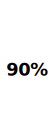
\includegraphics[height=3.9cm]{images/clustering/95.pdf}}
   & \subfloat[45 Clusters]{\includegraphics[width=3.9cm]{images/clustering/sl-95.pdf}} 
   & \subfloat[51 Clusters]{\includegraphics[width=3.9cm]{images/clustering/cl-95.pdf}}
   & \subfloat[47 Clusters]{\includegraphics[width=3.9cm]{images/clustering/al-95.pdf}} \\[-0.1in] % reducir la separacion entre filas 

% \textbf{90\%}
\subfloat{\includegraphics[height=3.9cm]{images/clustering/90.pdf}}
   & \subfloat[27 Clusters]{\includegraphics[width=3.9cm]{images/clustering/sl-90.pdf}} 
   & \subfloat[37 Clusters]{\includegraphics[width=3.9cm]{images/clustering/cl-90.pdf}}
   & \subfloat[29 Clusters]{\includegraphics[width=3.9cm]{images/clustering/al-90.pdf}} \\[-0.1in]

% \textbf{85\%}
\subfloat{\includegraphics[height=3.9cm]{images/clustering/85.pdf}}
   & \subfloat[22 Clusters]{\includegraphics[width=3.9cm]{images/clustering/sl-85.pdf}} 
   & \subfloat[22 Clusters]{\includegraphics[width=3.9cm]{images/clustering/cl-85.pdf}}
   & \subfloat[20 Clusters]{\includegraphics[width=3.9cm]{images/clustering/al-85.pdf}} \\[-0.1in]

% \textbf{80\%}
\subfloat{\includegraphics[height=3.9cm]{images/clustering/80.pdf}}
   & \subfloat[13 Clusters]{\includegraphics[width=3.9cm]{images/clustering/sl-80.pdf}} 
   & \subfloat[9 Clusters]{\includegraphics[width=3.9cm]{images/clustering/cl-80.pdf}}
   & \subfloat[7 Clusters]{\includegraphics[width=3.9cm]{images/clustering/al-80.pdf}} \\[-0.1in]

% \textbf{75\%}
\subfloat{\includegraphics[height=3.9cm]{images/clustering/75.pdf}}
   & \subfloat[9 Clusters]{\includegraphics[width=3.9cm]{images/clustering/sl-75.pdf}} 
   & \subfloat[5 Clusters]{\includegraphics[width=3.9cm]{images/clustering/cl-75.pdf}}
   & \subfloat[5 Clusters]{\includegraphics[width=3.9cm]{images/clustering/al-75.pdf}} \\[0in]    
\end{tabular}

\caption{Resultados experimento de Clustering de Tests por Similitud en Cobertura}\figlabel{ap-clustering}
\end{figure}
%================ 

\newpage
\par Luego de una inspección entre los distintos resultados, el parámetro de similitud interna mínima escogido fue de 85\%, ya que los tres resultados generan una cantidad de clusters razonable y con muy buena similitud interna. Entre las tres opciones, se descartó la opción (\emph{Single Link}, 85\%) ya que la mitad de sus clusters son unitarios (condición 3), y tampoco respeta la condición 2, ya que tiene un cluster con más de 30 tests, el siguiente en tamaño 18 (casi la mitad del primero) y el siguiente 10 (casi la mitad del tercero y un tercio del primero) y luego muchos clusters pequeños. 

% Tabla comparativa 3 mejores casos

%== Comparacion entre clusterings
\begin{figure}
\centering
\begin{tabular}{c}
\subfloat[Comparación de los tamaños de cada cluster]{\includegraphics[width=14cm]{images/clustering/comp-tamanos.pdf}} \\[2cm] 
\subfloat[Comparación de la similitud interna de cada cluster]{\includegraphics[width=14cm]{images/clustering/comp-sim-int.pdf}}
\end{tabular}
\caption{Análisis comparativo entre los dos mejores agrupamientos}

\footnotesize
\begin{tabular}{rl}
\textbf{Azul}: & \emph{Average Link}, 85\% \\
\textbf{Rojo}: & \emph{Complete Link}, 85\%
\end{tabular}
\figlabel{ap-comp-clus}
\end{figure}


\par Entre las dos alternativas restantes se realizó una comparación mas minuciosa. Por un lado, la alternativa (\emph{Complete Link}, 85\%) genera dos clusters más que (\emph{Average Link}, 85\%) (ver \figref{ap-clustering} (k) y (l)), los dos casos presentan igual número de clusters unitarios. La \figref{ap-comp-clus} muestra los gráficos comparativos según tamaño y similitud interna. En ambos gráficos los clusters están ordenados de izquierda a derecha según su tamaño (número de elementos) y en orden decreciente. 

\par La \figref{ap-comp-clus}(a) permite revisar la condición 2. Allí se aprecia que la mejor distribución de los tests se da en (\emph{Complete Link}, 85\%) ya que los clusters no difieren tanto en tamaño. Además en el caso de (\emph{Average Link}, 85\%) se observa un escenario similar al de (\emph{Single Link}, 85\%) con un cluster de gran tamaño, el siguiente la mitad del primero, y así sucesivamente. Inicialmente se pensó en el caso en que el cluster $C_{1,AL}$ del caso \emph{Average Link} fueran los clusters $C_{1,CL}$ y $C_{2,CL}$ de \emph{Complete Link} fusionados, pero luego de una inspección con TestSurgeon determinó que esto no era así y que de hecho los dos clusters $C_{1,CL}$ y $C_{2,CL}$ eran bastante distintos ya que la similitud entre sus elementos en general era menor al 80\% (menor que la $s_{min}$). 

\par Esta mejor distribución en el caso de \emph{Complete Link} se explica porque la métrica es más conservadora. Ya que los clusters fusionados en cada paso del algoritmo son los más cercanos considerando como distancia entre clusters los elementos más lejanos de cada cluster. Es decir los tests fusionados son realmente muy cercanos ya que la cota mínima de similitud interna es bastante exigente. En contraparte, \emph{Average Link}, al considerar los promedios de similitudes no toma en cuenta la varianza de similitudes que existen entre las parejas de tests de los clusters.

\par La \figref{ap-comp-clus}(b) permite revisar la condición 1. En este caso el contraste es aun mayor ya que en general los clusters de (\emph{Complete Link}, 85\%) son más homogéneos, es decir, sus elementos son más similares. Y el cluster más heterogéneo ($C_{11,CL}$) tiene una similitud interna de $89\%$ y es el único caso. Además el 60\% de los clusters formados tiene $s$ sobre el $92\%$ lo cual habla de clusters equilibrados en tamaño y muy similares entre ellos. Es decir en (\emph{Complete Link}, 85\%) además de reducir el número total de comparaciones, los pares de tests a comparar son entre sí muy similares (en cada cluster).

\par Finalmente, traduciendo lo anterior a número de comparaciones se tiene: (\emph{Average Link}, 85\%) = 648 comparaciones, y (\emph{Complete Link}, 85\%) con \textbf{405 comparaciones}. Por lo cual la configuración escogida es {\bf (\emph{Complete Link}, 85\%)}.

\section{Conclusión}

\par En conclusión se obtuvo una reducción de comparaciones que inicialmente eran 4.560 a 405. Luego del agrupamiento se descartó el 91\% de las comparaciones iniciales las cuales eran innecesarias puesto que la cobertura entre los elementos no daba lugar a un caso de interés. Esto significa una inmensa reducción de tiempo para el desarrollador y le permite enfocarse en los casos realmente interesantes donde existe la posibilidad de restructuración o refactorización. 





\chapter{Herramientas de Cobertura revisadas}\aplabel{review-test-coverage-tools}

\par A continuación se listan las herramientas de cobertura de test analizadas y comparadas con \emph{TestSurgeon}, con sus respectivas URL\footnote{Todas las URL fueron consultadas por última vez el día 12/08/2013} donde se pueden obtener.
\begin{description}
\item[Emma] [en línea] \textless\url{http://emma.sourceforge.net/}\textgreater  \\
\item[EclEmma] [en línea] \textless\url{http://www.eclemma.org}\textgreater  \\
\item[JCover] [en línea] \textless\url{http://www.mmsindia.com/JCoverSampleScreen.html}\textgreater  \\
\item[GroboCodeCoverage] [en línea] \textless\url{http://groboutils.sourceforge.net/codecoverage/index.html}\textgreater  \\
\item[JCoverage] [en línea] \textless\url{http://maven.apache.org/maven-1.x/plugins/jcoverage/}\textgreater   $\quad$ Desafortunadamente, ya no sigue siendo desarrollado \\
\item[Parasoft JTest] [en línea] \textless\url{http://www.parasoft.com/jsp/products/jtest.jsp?itemId=14}\textgreater  \\
\item[Purity Plus] [en línea] \textless\url{http://www-03.ibm.com/software/products/us/en/purifyplus}\textgreater  \\
\item[Semantic Designs] [en línea] \textless\url{http://www.semdesigns.com/Products/TestCoverage/}\textgreater  \\
\item[TCAT] [en línea] \textless\url{http://www.testworks.com/Products/TCAT-Java/tcat.java.html}\textgreater  \\
\item[Quilt] [en línea] \textless\url{http://quilt.sourceforge.net/quilt-0.4/}\textgreater   \\
\item[NoUnit] [en línea] \textless\url{http://nounit.sourceforge.net/}\textgreater   \\
\item[InsectJ] [en línea] \textless\url{http://insectj.sourceforge.net}\textgreater  \\
\item[Hansel] [en línea] \textless\url{http://hansel.sourceforge.net/}\textgreater  \\
\item[Gretel] [en línea] \textless\url{http://www.cs.uoregon.edu/research/perpetual/dasada/Software/Gretel/}\textgreater  \\
\item[Jester] [en línea] \textless\url{http://jester.sourceforge.net/}\textgreater  \\
\item[JVMDI Code Coverage] [en línea] \textless\url{http://jvmdicover.sourceforge.net/}\textgreater  \\
\item[JBlanket] [en línea] \textless\url{http://csdl.ics.hawaii.edu/research/jblanket/}\textgreater  \\
\item[Coverlipse] [en línea] \textless\url{http://coverlipse.sourceforge.net}\textgreater  \\
\item[Koalog] [en línea] \textless\url{http://freecode.com/projects/kcc}\textgreater  \\
\item[Cobertura] [en línea] \textless\url{http://cobertura.sourceforge.net}\textgreater  \\
\item[Mojo] [en línea] \textless\url{http://mojo.codehaus.org/cobertura-maven-plugin/}\textgreater  \\
\item[Thucydides] [en línea] \textless\url{http://docs.codehaus.org/display/SONAR/Thucydides+Plugin}\textgreater  
\end{description}






\end{document}
